\documentclass[12pt,fleqn]{article}\usepackage{../common}
\begin{document}
Yaklasiksal SVD ile Tavsiye Sistemleri

Gecmis verilere bakarak bir kullanicinin hic seyretmedigi bir filme nasil
not verecegini tahmin etmek unlu Netflix yarismasinin konusuydu. Onceki bir
yazi {\em SVD, Toplu Tavsiye}'de benzer bir veri seti Movielens uzerinde
SVD uygulayarak once boyut azaltmistik, azaltilmis boyut uzerinden yeni (o
film icin notu bilinmeyen) bir kullanicinin diger mevcut kullanicilara
mesafesini hesaplamis, ve boylece begeni acisindan en cok benzedigi diger
kullaniciyi bulmustuk (birkac tane de bulunabilir). Bu kullanicinin bir
film icin verdigi notu yeni kullanici icin tahmin olarak baz almistik.

SVD uygulamanin tek yontemi bu degil. Netflix yarismasinda kullanilan [1]
bir yaklasim soyle; alttaki SVD ayristirmasina bakalim,

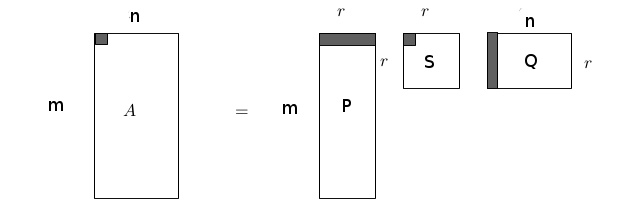
\includegraphics[height=4cm]{svdapprox_1.png}

1. kullanicini 1. filme verdigi not ustte koyu gosterilen satirlarin
carpimi ile oluyor, eger ufak harfler ve kullanici (user) icin $u$, film
icin $i$ indisini kullanirsak, ve $q,p$ vektorlerini $Q,P$ matrislerinin
sirasiyla kolon ve satirlarini gostermek icin kullanirsak, ayristirma
sonrasi begeni degeri (onemli bir kismi daha dogrusu) $q_i^Tp_u$
carpimindadir. Carpim icinde $S$'ten gelecek tekil degeri (singular value)
ne olacak?  Simdi formulasyonu biraz degistirelim, bu degeri carpim disina
alarak birkac toplam olarak gosterebiliriz. Bu toplamlar mesela bir
kullanicinin ne kadar yanli (bias) not verdigini, ya da bir filmin kabaca,
ortalama nasil not almaya meyilli oldugunu modelleyebilirler (ki bu da bir
yanlilik olcusu). Ayrica tum filmlere verilen notlarin yanliligi da
olculebilir. Tum bunlari bir araya koyarsak, bir begeni notunu tahmin
edecek formul soyle gosterilebilir,

$$
\hat{r}_{ui} = \mu + b_i + b_u + q_i^Tp_u
$$

$\mu$ bir skalar, tum filmlere verilen ortalamayi gosteriyor, ki tum
begenilerin sayisal ortalamasi uzerinden basit bir sekilde hizla
hesaplanabilir. $\hat{r}_{ui}$'ya bir tahmin dedik cunku modelimizdeki
vektorlerin degerlerini bulduktan sonra (egitim verisiyle bu hesabi
yapacagiz) modeli kullanarak gercek not $r_{ui}$ icin bir
tahmin yapmaya ugrasacagiz.

Yanlilik hakkinda bazi ornekler vermek gerekirse, diyelim ki kullanici Bob
not verirken yuksek seviyede oy vermeye meyilli. Bu durumda bu kullanicinin
ortalama hatta dusuk oy vermesi onun bir filmden hakikaten hic
hoslanmadigini sinyalleyebilir. Ya da mesela bir film, genellikle ortalama
oy almaktadir, bu durumda ona cok iyi not veren bir kisinin bu filmi cok
begendigi ortaya cikar. Modeldeki yanlilik parametreleri bu durumu
saptayabilirler.

Egitim

Egitim icin ne yapmali? Minimize edecegimiz bir hedef fonksiyonu kuralim,
ki cogunlukla bu karesi alinmis hata ile olur. Mesela gercek not
$r_{ui}$ degerinden tahmin notu $\hat{r}_{ui}$'yi cikartip karesini
alabiliriz. Bu islemi tum $u,i$'ler icin yaparak sonuclari toplariz, ve bu
toplami minimize etmeye ugrasabiliriz. Yani


$$
\min_{b*,q*,p*} \sum_{u,i} (r_{ui} - \hat{r}_{ui})^2 + 
\lambda (b_i^2 + b_u^2 + ||q_i||^2 + ||p_u||^2)
$$

$$
= \min_{b*,q*,p*} \sum_{u,i} (r_{ui} - \mu - b_i - b_u - q_i^Tp_u)^2 + 
\lambda (b_i^2 + b_u^2 + ||q_i||^2 + ||p_u||^2)
$$

Kisaltma olarak $e_{ui}$ tanimlayalim, bu faydali olabilir, formuldeki ilk
parantez icindeki kisimda $e_{ui}$ kullanmak uzere,
$$ e_{ui} := r_{ui} - \hat{r}_{ui} $$

$\lambda$ ile carpilan bolum regularizasyon icin. Istatistik, yapay
ogrenim, optimizasyon alanlarinda modelimizin asiri uygunluk (overfitting)
yapmasini engellemek icin regularizasyon kullanilir, bunun icin istedigimiz
degiskenlerin fazla buyumesini cezalandiririz, ustteki minimizasyon
modelinde bu ceza icin tum degerlerin buyuklugunu (magnitude) hesapladik
-skalar degerlerin karesini, vektor degerlerinin kare norm'unu alarak- ve
bu buyuklukleri bizim disaridan set edebilecegimiz bir sabitle carpilmasi
uzerinden minimizasyon problemine direk dahil ettik. Boylece bu buyuklukler
formulasyona dahil oldular ve azaltilma hedefinin bir parcasi haline
geldiler. Yani hem $e_{ui}^2$ hem de hatayi olusturan degerlerin kendileri
minimize edilecek.

Rasgele Gradyan Inisi (Stochastic Gradient Descent -SGD-)

Modeli nasil minimize ederiz? Bu model konveks (convex) degil, ki
konvekslik bilindigi gibi fonksiyonun duzgun bir cukur gibi oldugu
problemlerdir, herhangi bir noktadan baslarsiniz, gradyani hesaplarsiniz,
ve bu gradyan hep optimal inis noktasini gosterir cunku cukurda ``takilip
kalabileceginiz'', ``yerel minimumlar'' mevcut degildir . Bizim
problemimizde $q_i^Tp_u$ var, bu degiskenlerin ikisi de bilinmiyor, ve bu
carpimin karesi alindigi icin genel karesellligi (quadratic) kaybetmis
oluyoruz. Fakat yine de SGD bu problemi cozebiliyor. Bunun sebeplerini, SGD
SVD'nin hikayesiyle beraber yazinin sonunda bulabilirsiniz. 

SGD icin gradyanlar lazim, her degisken icin minimizasyon toplami icindeki
kismin (bu kisma $E$ diyelim) ayri ayri kismi turevini almak lazim. Mesela
$b_u$ icin

$$ \frac{\partial E}{\partial b_u}  = -2e_{ui} + 2 \lambda b_u
$$

Gradyan her zaman en yuksek cikisi gosterir, o zaman hesapsal algoritma
onun tersi yonune gitmelidir. Bu gidisin adim buyuklugunu kontrol etmek
icin disaridan bizim belirledigimiz bir $\gamma$ sabiti ile carpim
yapabiliriz, ve bir numara daha, sabit 2 degerlerinin $\gamma$ icinde
eritilebilecegini farzederek onlari sileriz. Yani adim $\gamma(e_{ui} - \lambda b_u)$ 
haline geldi. Bir dongu icinde eski $b_u$ bulunacak,
gordugumuz yonde adim atilacak, yani adim onceki degere toplanacak, ve yeni
deger elde edilecek. Diger degiskenler icin de ayni islemi yaparsak, sonuc 
soyle,

$$ b_u \leftarrow b_u + \gamma (e_{ui} - \lambda \cdot b_u) $$

$$ b_i \leftarrow b_i + \gamma (e_{ui} - \lambda \cdot b_i) $$

$$ q_i \leftarrow q_i + \gamma (e_{ui}\cdot p_u - \lambda \cdot q_i) $$

$$ p_u \leftarrow p_u + \gamma (e_{ui}\cdot q_i - \lambda \cdot p_u) $$

Her degisken icin baslangic noktasi rasgele olarak secilebilir, ki
$\gamma,\lambda$ sabitleri ile beraber bu baslangic noktalari icin en iyi
degerler deneme/ yanilma ya da capraz saglama (crossvalidation) ile
bulunabilir.

Rasgelelik, aynen {\em Lojistik Regresyon} orneginde oldugu gibi verinin
rasgeliliginden geliyor, her veri noktasini teker teker sirayla isliyoruz
aslinda fakat bu ``siranin'' rasgele oldugunu farzettigimiz icin ozyineli 
algoritmamiz rasgelelik elde ediyor. Python kodu altta, egitim icin kod
sadece bir kere verinin uzerinden geciyor. Basa donup birkac kere (hatta
yuzlerce) veriyi isleyenler de oldu.

\inputminted[fontsize=\footnotesize]{python}{ssvd.py}

Kodun onemli bir ozelligi sudur, bos yani \verb!nan! degeri iceren notlar
egitim sirasinda atlanir. SGD seyrek verilerle de isleyebilen bir egitim
yontemidir. Bu durumda verinin seyrekligi (sparsity) bizim icin cok
faydali, cunku o veri noktalarina bakilmayacak, \verb!row.notnull()! ile
bos olmayan ogelerin indis degerlerini aliyoruz.

Basit bir ornek

\begin{minted}[fontsize=\footnotesize]{python}
import pandas as pd
import ssvd
d =  np.array(
[[  5.,   5.,   3.,  nan,   5.,   5.],
 [  5.,  nan,   4.,  nan,   4.,   4.],
 [ nan,   3.,  nan,   5.,   4.,   5.],
 [  5.,   4.,   3.,   3.,   5.,   5.],
 [  5.,   5.,  nan,  nan,  nan,   5.]
])
data = pd.DataFrame (d, columns=['0','1','2','3','4','5'],
       index=['Ben','Tom','John','Fred','Bob'])
mu,b_u,b_i,q_i,p_u = ssvd.ssvd(data,rank=3)
print mu
print 'b_u',b_u
print 'b_i',b_i
print 'q_i',q_i
print 'p_u',p_u
u = 4; i = 2 # Bob icin tahmin yapalim
r_ui_hat = mu + b_i[i] + b_u[u] + np.dot(q_i[:,i].T,p_u[u,:])
print r_ui_hat
\end{minted}

\begin{verbatim}
rank 3
4.31388888889
b_u [ 0.05129388  0.01927226  0.0206893   0.0065487   0.06568321]
b_i [ 0.07820389  0.01958841 -0.03217881  0.01561187  0.04071886  0.07140383]
q_i [[ 0.03132989  0.02957741  0.02802317  0.02951804  0.0301854   0.03108419]
 [ 0.03132989  0.02957741  0.02802317  0.02951804  0.0301854   0.03108419]
 [ 0.03132989  0.02957741  0.02802317  0.02951804  0.0301854   0.03108419]]
p_u [[ 0.03053543  0.03053543  0.03053543]
 [ 0.0295772   0.0295772   0.0295772 ]
 [ 0.02963018  0.02963018  0.02963018]
 [ 0.02921864  0.02921864  0.02921864]
 [ 0.03100583  0.03100583  0.03100583]]
4.34999993855
\end{verbatim}

Test Etmek

Test verisi olusturmak icin egitim verisinde rasgele olarak bazi notlari
sectik, bunlari bir kenara kaydederek onlarin ana matris icindeki degerini
sildik (yerine \verb!nan!  koyarak), ve bir kismi silinmis yeni bir egitim
matrisi yarattik, \verb!create_training_test! islevinde bu gorulebilir. Bu
islevde her kullanicidan sadece bir tane not verisi aliyoruz, ve bunu
sadece belli bir sayida, \verb!collim! kadar, not vermis kullanicilar icin
yapiyoruz, ki boylece az sayida not vermis kullanicilarin verisini silmemis
oluyoruz. Ayrica belli miktarda, \verb!rowlim! kadar test noktasi elde
edince is bitti kabul ediyoruz. Test verisi yaratmak icin \%80-\%20 gibi
bir ayrim yapmadik, yani egitim verisindeki tum kullanicilari ve onlarin
neredeyse tum verisini egitim icin kullaniyoruz.

Movielens verisine gelelim. {\em SVD, Toplu Tavsiye} yazisindaki
\verb!movielens_prep.py! ile gerekli egitim dosyasi uretildigini
farzederek,

\begin{minted}[fontsize=\footnotesize]{python}
import pandas as pd, os
df = pd.read_csv("%s/Downloads/movielens.csv" % os.environ['HOME'] ,sep=';')
print df.shape
df = df.ix[:,1:3700] # id kolonunu atla,
df.columns = range(3699) # kolon degerlerini tekrar indisle
print df.shape
\end{minted}

\begin{verbatim}
(6040, 3731)
(6040, 3699)
\end{verbatim}

Egitim ve test verisi yaratiyoruz,

\begin{minted}[fontsize=\footnotesize]{python}
import ssvd
df_train, test_data = ssvd.create_training_test(df,rowlim=500,collim=300)
print len(test_data)
\end{minted}

\begin{verbatim}
501
\end{verbatim}

Egitim

\begin{minted}[fontsize=\footnotesize]{python}
import ssvd
mu,b_u,b_i,q_i,p_u = ssvd.ssvd(df_train,rank=25)
print 'mu',mu
\end{minted}

\begin{verbatim}
rank 25
mu 3.23835007474
\end{verbatim}

Test

\begin{minted}[fontsize=\footnotesize]{python}
rmse = 0; n = 0
for u,i,real in test_data:
    r_ui_hat = mu + b_i[i] + b_u[u] + np.dot(q_i[:,i].T,p_u[u,:])
    rmse += (real-r_ui_hat)**2
    n += 1
print "rmse", np.sqrt(rmse / n)
\end{minted}

\begin{verbatim}
rmse 0.903347878156
\end{verbatim}

Sonuc oldukca iyi.

Formulasyonun Hikayesi

SGD SVD'nin hikayesi soyle. Yil 2009, Netflix Yarismasi [11]
katilimcilarindan Simon Funk (gercek adi Brandyn Webb) SGD SVD yaklasimini
kodlayip veri uzerinde isletince birden bire siralamada ilk 3'e firlar;
Webb artik cok unlu olan blog yazisinda [1] yaklasimi detayiyla paylasip
forum'da haberini verince bu haber tam bir bomba etkisi yaratir. Pek cok
kisi yaklasimi kopyalar, hatta kazanan BellKor urununde Webb'in SVD
yaklasiminin kullanildigi biliniyor.

Bu metotun kesfi hangi basamaklardan gecti? Beni meraklandiran minimizasyon
formulasyonun konveks olmamasiydi -- genellikle optimizasyon problemlerinde
konveksligin mevdudiyeti aranir, cunku bu durumda sonuca yaklasmak
(convergence) icin bir garanti elde edilir. Bu durumda konvekslik
yoktu. Biraz arastirinca Bottou ve LeCunn gibi arastirmacilarin yazilarina
ulastik [4]. Onlara gore konvekslik olmamasi yapay ogrenim
arastirmacilarini korkutmamali, eger sayisal (empirically) isleyen bir
algoritma var ise, teorik ispat gelene kadar bu metotun kullanilmasinda
sakinca yoktur.

Fakat boyle buluslarda yine de bazi garantiler temel alinmis olabilir,
arastirmaci tamamen baliklama atlayis yapmaz. Webb'in kendisine bu sorulari
sorduk ve bize bulusun hangi seviyelerden gectigini anlatti. Geriye
sariyoruz, Webb Netflix'den cok once yapay sinir aglarini arastirmaktadir,
ve Sanger, Oja'nin [5,6] yayinlarini baz alarak kurdugu bir YSA icin bir
cozum buldugunu farkeder. Sayisal cozumde ozdeger/vektor bulmaya yarayan
Ustel Metotun (power method) bir seklini kullanmistir, ki Sanger'in Genel
Hebbian Algoritmasinin (GHA) ustel metot ile baglantilari var, ve bu GHA
yayininda ``egitilince'' ozdeger/vektor ve PCA hesabi yapabilen bir YSA'dan
bahsediliyor. Daha onemlisi GHA 1 olasilikla (yani kesin) bu sonuclara
erisebiliyor.

Daha sonra Webb bu cozumu arkadasi Gorrell ile tartisirken Gorrell ona
problem formulasyonunun SVD olarak gorulebilecegini soyler. Bilindigi gibi
ozdeger/vektor hesabi ile SVD yakin akraba sayilir. Ikili bu baglamda
birkac yayin da yaparlar. Daha sonra Netflix yarismasi basladiginda Webb
cozum icin gradyan baz alarak SGD kullanabilecegini farkediyor, ki SGD ile
ustel metot arasinda teorik baglanti var [7]. Ve sonuc olarak SGD SVD
metotu ortaya cikiyor.

Tabii ki ``SGD SVD ne kadar SVD sayilir?'' gibi bir soru sorulabilir. Evet,
regularizasyon bazi gayri-lineerlikleri probleme sokar, zaten bu cozumu
``yaklasiksal'' yapan kisim da budur. Fakat belli sartlarda, regularizasyon
olmasa cozum tam SVD olacaktir. Bu bulusun puf noktasi bu bilgide, ve
ustteki teorik benzerliklerde, onlari biliyor olmakta yatiyor. Eger bunlar
biliniyor ise, ve saglam lineer cebir bilgisi ile gerektigi zaman onlari ne
kadar esnetebilecegimizi biliriz. Konu hakkindaki daha fazla detay surada
[10] bulunabilir.

Kaynaklar

[1] \url{http://sifter.org/~simon/journal/20061211.html}

[2] Koren, Bell, {\em Recommender Systems Handbook},
\url{http://www.cs.bme.hu/nagyadat/Recommender_systems_handbook.pdf}

[3] \url{http://www2.research.att.com/~volinsky/papers/ieeecomputer.pdf}

[4] \url{http://www.cs.nyu.edu/~yann/talks/lecun-20071207-nonconvex.pdf}

[5] \url{http://courses.cs.washington.edu/courses/cse528/09sp/sanger_pca_nn.pdf}

[6] \url{http://users.ics.aalto.fi/oja/Oja1982.pdf}

[7] \url{http://arxiv.org/pdf/1308.3509}

[8] \url{http://www.maths.qmul.ac.uk/~wj/MTH5110/notes/MAS235_lecturenotes1.pdf}

[9] \url{http://heim.ifi.uio.no/~tom/powerandqrslides.pdf}

[10] \url{http://math.stackexchange.com/questions/649701/gradient-descent-on-non-convex-function-works-but-how}

[11] Netflix Odulu, \url{http://www.netflixprize.com}

\end{document}
